% chapters/softstart.tex
% generated from soft_starter.tex
\chapter{Thyristor soft starters}
\label{ch:softstart}
\begin{chapabstract}
This note gives an engineering overview of thyristor-based soft starters
(reduced-voltage solid-state starters) for medium and large induction motors.
It covers the motor starting problem, the phase-angle control principle,
the main circuit topologies (in-line, inside-delta, medium-voltage series
strings), the power levels at which soft starters are typically applied,
device selection, thermal duty, and the interaction with the supply during
the starting ramp. A dedicated section discusses the role and sizing of
snubbers in these applications: $\mathrm{d}v/\mathrm{d}t$ limitation of
phase-control thyristors, damping of commutation transients, dynamic voltage
sharing in series-connected strings, and coordination with metal-oxide
varistors. A worked sizing example for a \SI{690}{\volt}, \SI{1}{\mega\watt}
starter is included.
\end{chapabstract}

%=====================================================================
\section{Introduction}
%=====================================================================

A three-phase squirrel-cage induction motor connected directly to the line
(direct-on-line, DOL, starting) draws a starting current of typically 5 to 8
times its rated current at a poor power factor, and develops a starting
torque that is fixed by the motor design rather than by the needs of the
driven load. For small motors on stiff supplies this is acceptable. For
motors in the hundreds of kilowatts to tens of megawatts range, DOL starting
causes:

\begin{itemize}
  \item severe voltage dips on the supply, which may violate utility
        connection agreements or trip other loads;
  \item high electrodynamic and thermal stress in the stator winding and in
        the rotor cage, reducing motor life when starts are frequent;
  \item mechanical shock in the driven equipment (couplings, gearboxes,
        belts) and hydraulic transients (water hammer) in pump systems.
\end{itemize}

The soft starter is the simplest solid-state answer to this problem. It is a
three-phase AC voltage controller built with anti-parallel phase-control
thyristors, inserted between the line and the motor. By delaying the firing
of the thyristors with respect to the line voltage, the fundamental voltage
applied to the motor is reduced in a controlled way, and with it the starting
current and torque. Once the motor has reached rated speed the thyristors are
fired continuously (or the starter is bypassed by a contactor) and the motor
runs directly on the line. The soft starter therefore controls only the
\emph{starting and stopping transients}; unlike a variable-frequency drive
(VFD) it provides no continuous speed control.

Soft starters are attractive at high power precisely because the power
circuit is minimal: two thyristors per phase, no DC link, no fast switching,
no output filter. The cost, volume, and losses are a small fraction of those
of a VFD of equal rating, which is why soft starters remain the standard
solution for fixed-speed pumps, fans, compressors, conveyors, crushers, and
mills from a few tens of kilowatts up to tens of megawatts.

%=====================================================================
\section{The Starting Problem}
%=====================================================================

For a squirrel-cage motor the locked-rotor current $I_\mathrm{LR}$ is
essentially determined by the total leakage impedance and is nearly
independent of the mechanical load:
\begin{equation}
  I_\mathrm{LR} \approx \frac{V_\mathrm{ph}}
  {\sqrt{(R_s + R_r')^2 + (X_{\sigma s} + X_{\sigma r}')^2}}
  \approx (5\ldots8)\,I_N .
\end{equation}
At reduced stator voltage the current scales linearly with voltage, while
the torque at any given slip scales with the voltage squared:
\begin{equation}
  I(s) \propto V, \qquad T(s) \propto V^2 .
  \label{softstart:eq:v2}
\end{equation}
Equation~\eqref{softstart:eq:v2} is the fundamental trade-off of every reduced-voltage
starting method: halving the starting current quarters the starting torque.
A soft start is therefore only possible if the load torque during
acceleration is well below the motor torque at the reduced voltage. This is
the case for centrifugal loads (pumps, fans), where the load torque grows
approximately with the speed squared, and it is the reason why soft starters
are so common in exactly those applications. High-breakaway loads (loaded
conveyors, positive-displacement compressors, mills with material) require a
higher current limit or a different starting method.

Figure~\ref{softstart:fig:torquespeed} illustrates the effect: the motor torque--speed
curve is scaled by $(V/V_N)^2$, and the intersection with the load curve
defines the accelerating torque available during the ramp.

\begin{figure}[htb]
\centering
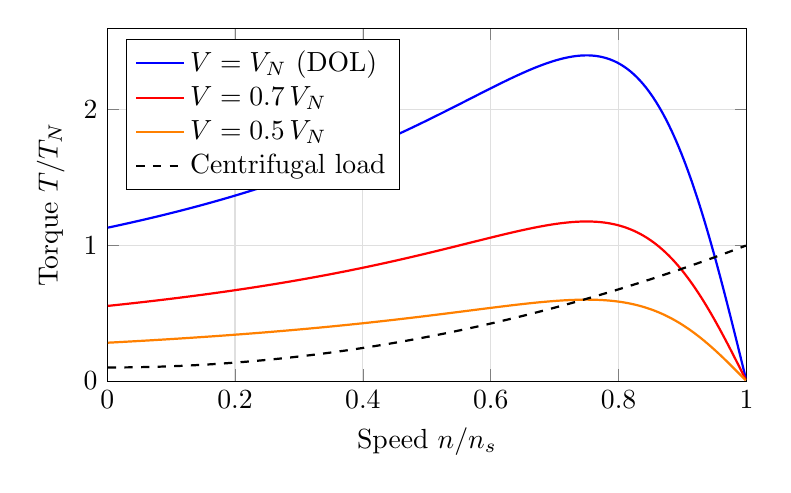
\begin{tikzpicture}
\begin{axis}[
  width=0.8\textwidth, height=0.5\textwidth,
  xlabel={Speed $n/n_s$}, ylabel={Torque $T/T_N$},
  xmin=0, xmax=1, ymin=0, ymax=2.6,
  legend pos=north west, legend cell align=left,
  grid=both, grid style={gray!25},
  domain=0.001:0.999, samples=200]
% Kloss curve: T = 2*Tb/(s/sb+sb/s), Tb=2.4 TN, sb=0.25, s=1-x
\addplot[thick,blue]  {2*2.4/(((1-x)/0.25)+(0.25/(1-x)))};
\addlegendentry{$V = V_N$ (DOL)}
\addplot[thick,red]   {0.49*2*2.4/(((1-x)/0.25)+(0.25/(1-x)))};
\addlegendentry{$V = 0.7\,V_N$}
\addplot[thick,orange]{0.25*2*2.4/(((1-x)/0.25)+(0.25/(1-x)))};
\addlegendentry{$V = 0.5\,V_N$}
\addplot[thick,dashed,black] {0.1+0.9*x^2};
\addlegendentry{Centrifugal load}
\end{axis}
\end{tikzpicture}
\caption{Induction motor torque--speed curves at reduced voltage
($T \propto V^2$) and a centrifugal load curve. At $0.5\,V_N$ the motor
still accelerates a centrifugal load, but would stall against a
constant-torque load of rated value.}
\label{softstart:fig:torquespeed}
\end{figure}

%=====================================================================
\section{Overview of Reduced-Voltage Starting Methods}
%=====================================================================

Table~\ref{softstart:tab:methods} places the soft starter among the classical
alternatives. The electromechanical methods (star--delta, autotransformer,
reactor) reduce the voltage in one or two fixed steps; the transition
between steps produces current and torque transients that can approach DOL
values. The soft starter replaces the steps by a continuous, closed-loop
controlled ramp, and adds soft stopping, which no electromechanical method
provides.

\begin{table}[htb]
\centering
\caption{Comparison of starting methods for a motor with
$I_\mathrm{LR} = 6\,I_N$.}
\label{softstart:tab:methods}
\begin{tabular}{@{}lllll@{}}
\toprule
Method & Line current & Torque & Transients & Relative cost \\
\midrule
Direct on line      & $6\,I_N$            & $T_\mathrm{LR}$        & none (single shock) & lowest \\
Star--delta         & $2\,I_N$            & $T_\mathrm{LR}/3$      & severe at changeover & low \\
Autotransformer     & $(2\ldots4)\,I_N$   & $k^2\,T_\mathrm{LR}$   & moderate at steps    & medium \\
Series reactor      & $(3\ldots4.5)\,I_N$ & $k^2\,T_\mathrm{LR}$   & moderate             & medium \\
Soft starter        & $(2\ldots4.5)\,I_N$, adjustable & $\propto V^2$, ramped & none & medium \\
VFD                 & $\leq I_N$          & up to $T_N$ at all speeds & none & highest \\
\bottomrule
\end{tabular}
\end{table}

%=====================================================================
\section{The Thyristor Soft Starter}
%=====================================================================

\subsection{Phase-angle control principle}

The power circuit is a three-phase AC voltage controller: one pair of
anti-parallel phase-control thyristors per phase
(Fig.~\ref{softstart:fig:topology}). Each thyristor is fired with a delay angle
$\alpha$ measured from the zero crossing of its anodic voltage and turns off
naturally at the following current zero (line commutation). Increasing
$\alpha$ shortens the conduction interval and reduces the fundamental
component of the motor voltage. Because the motor is an inductive load with a
back-EMF, the relation between $\alpha$ and the fundamental voltage is
nonlinear and load-dependent; practical starters therefore close a control
loop around measured current rather than commanding a voltage directly.

\begin{figure}[htb]
\centering
\begin{circuitikz}[scale=0.9, transform shape]
% Phase A
\draw (0,5.6) node[left]{L1} to[short] (1.2,5.6);
\draw (1.2,5.6) -- (1.2,6.2) to[Ty] (3.2,6.2) -- (3.2,5.6);
\draw (1.2,5.6) -- (1.2,5.0);
\draw (3.2,5.0) to[Ty] (1.2,5.0);
\draw (3.2,5.0) -- (3.2,5.6);
\draw (3.2,5.6) to[short] (6.4,5.6);
% Phase B
\draw (0,2.8) node[left]{L2} to[short] (1.2,2.8);
\draw (1.2,2.8) -- (1.2,3.4) to[Ty] (3.2,3.4) -- (3.2,2.8);
\draw (1.2,2.8) -- (1.2,2.2);
\draw (3.2,2.2) to[Ty] (1.2,2.2);
\draw (3.2,2.2) -- (3.2,2.8);
\draw (3.2,2.8) to[short] (6.4,2.8);
% Phase C
\draw (0,0) node[left]{L3} to[short] (1.2,0);
\draw (1.2,0) -- (1.2,0.6) to[Ty] (3.2,0.6) -- (3.2,0);
\draw (1.2,0) -- (1.2,-0.6);
\draw (3.2,-0.6) to[Ty] (1.2,-0.6);
\draw (3.2,-0.6) -- (3.2,0);
\draw (3.2,0) to[short] (6.4,0);
% Bypass contactor on each phase (dashed)
\draw[dashed] (4.0,5.6) -- (4.0,7.0) to[nos] (5.6,7.0) -- (5.6,5.6);
\draw[dashed] (4.0,2.8) -- (4.0,4.2) to[nos] (5.6,4.2) -- (5.6,2.8);
\draw[dashed] (4.0,0) -- (4.0,1.4) to[nos] (5.6,1.4) -- (5.6,0);
\node[align=center] at (4.8,7.6) {bypass\\contactor};
% Motor
\draw (6.4,5.6) -- (7.2,5.6) -- (7.6,3.2);
\draw (6.4,2.8) -- (7.6,2.8);
\draw (6.4,0) -- (7.2,0) -- (7.6,2.4);
\draw (8.1,2.8) circle (0.55) node {M};
\draw (7.6,3.2) -- (7.66,3.05);
\draw (7.6,2.4) -- (7.66,2.55);
\end{circuitikz}
\caption{In-line three-phase soft starter: one anti-parallel pair of
phase-control thyristors per phase, with optional bypass contactor closed
after run-up.}
\label{softstart:fig:topology}
\end{figure}

Two properties of this circuit shape the whole design:

\begin{enumerate}
  \item \textbf{Line commutation.} The thyristors never interrupt current;
        they stop conducting at natural current zeros. The
        $\mathrm{d}i/\mathrm{d}t$ at turn-on and the reverse recovery are
        mild compared to inverter service, which is why standard
        phase-control (converter-grade) thyristors are used, not fast
        thyristors.
  \item \textbf{Discontinuous, asymmetric conduction.} During the ramp the
        phase currents are non-sinusoidal and may be discontinuous. Gating
        must use pulse trains (or long back-porch pulses) so that a
        thyristor is re-fired if its current attempts to restart within the
        intended conduction interval.
\end{enumerate}

\subsection{Topology variants}

\paragraph{In-line (six thyristors).} The standard arrangement of
Fig.~\ref{softstart:fig:topology}. Each pair carries the full line current and blocks
line-to-line voltage levels. This is the topology used at high power and the
only one used at medium voltage.

\paragraph{Inside-delta (six thyristors, six motor leads).} If all six
winding terminals are available, the pairs can be placed in series with each
delta winding. Each pair then carries only the winding current,
$I_\mathrm{line}/\sqrt{3} \approx 0.58\,I_\mathrm{line}$, allowing a smaller
starter frame for a given motor. The wiring is more complex and a wiring
error (e.g., swapped leads) can produce large uncontrolled currents, so this
variant is mostly found in LV retrofit applications.

\paragraph{Two-phase controlled (four thyristors).} One phase is connected
solidly and only two phases are controlled. This saves two devices but
produces asymmetric currents and a torque pulsation during the ramp. It is
restricted to small LV starters and is not used in the high-power range
considered here.

\paragraph{Bypass.} Almost all modern starters close a bypass contactor once
the motor has reached full voltage. This removes the thyristor conduction
losses (roughly $3 \times V_{T0} I_\mathrm{avg}$ plus resistive terms, i.e.,
kilowatts at megawatt motor ratings), shrinks the cooling system, and lets
the thermal design be based on the \emph{starting duty} only. The thyristors
must still be rated to carry the start current for the ramp duration and to
withstand the prospective short-circuit current until protection clears.

\subsection{Control functions}

Typical control features of an industrial soft starter:

\begin{itemize}
  \item \textbf{Voltage ramp:} open-loop ramp of the firing angle from an
        initial voltage (30--60\,\% $V_N$) to full voltage in an adjustable
        time (typically 2--60\,\si{\second}).
  \item \textbf{Current limit:} closed-loop regulation of the RMS line
        current to a set value, typically $(2\ldots4.5)\,I_N$, during
        acceleration. This is the mode normally used at high power, because
        it makes the supply loading predictable.
  \item \textbf{Kick start:} a short (0.1--1\,\si{\second}) pulse of higher
        voltage to break away high-stiction loads before the ramp.
  \item \textbf{Soft stop:} a controlled voltage ramp-down (10--60\,\si{\second}),
        essential in pumping systems to avoid check-valve slam and water
        hammer.
  \item \textbf{Protections:} electronic overload (thermal model of the
        motor), locked rotor, phase loss and phase reversal, thyristor
        failure (shorted SCR detection), starter over-temperature.
\end{itemize}

The implementation of these functions --- synchronization, firing logic, and
the control loop --- is discussed in Section~\ref{softstart:sec:control}.

%=====================================================================
\section{Control and Firing Architecture}
\label{softstart:sec:control}
%=====================================================================

\subsection{Firing infrastructure: the six-pulse bridge heritage}

The gating infrastructure of a soft starter is essentially that of a
line-commutated six-pulse (B6) thyristor bridge, and early industrial soft
starters were in fact built around rectifier firing boards. The common
elements are:

\begin{itemize}
  \item \textbf{Line synchronization:} a PLL (or filtered zero-crossing
        detector) locked to the supply provides the phase reference; it must
        reject the commutation notches and harmonic distortion that the
        starter itself injects during the ramp.
  \item \textbf{Six delay channels:} one firing-angle counter per thyristor,
        loaded from the common angle command and started at the reference
        instant of the corresponding device. The firing order is a ring
        counter advancing in \ang{60} steps, exactly as in a B6 bridge
        (for phase sequence L1--L2--L3:
        T1$^{+}$, T3$^{-}$, T2$^{+}$, T1$^{-}$, T3$^{+}$, T2$^{-}$, where
        $+/-$ denote the two devices of each anti-parallel pair).
  \item \textbf{Double pulsing:} with the standard three-wire connection
        (no neutral), a phase current can only close through another phase.
        A thyristor fired alone therefore cannot conduct: at every firing
        instant the incoming device \emph{and} the appropriate device of a
        second phase must be gated together --- the exact analogue of the
        second (repeat) pulse in a B6 bridge. Equivalently, each gate
        command is issued twice, \ang{60} apart.
  \item \textbf{Pulse trains with back-porch:} because conduction is
        discontinuous during the ramp, a device whose current attempts to
        restart within its intended conduction interval must be re-fired.
        Gating therefore uses high-frequency pulse trains (or long pulses
        with a sustained back-porch current above $I_{GT}$) covering the
        whole interval, transmitted through pulse transformers at LV and
        fiber-optic links to local gate units at MV.
\end{itemize}

\subsection{Differences from the rectifier}

Three points prevent a literal reuse of the rectifier control law:

\paragraph{Angle reference.} In a B6 bridge, $\alpha$ is measured from the
natural commutation points (the crossings of the line-to-line voltages). In
the AC controller each thyristor is referred to the zero crossing of
\emph{its own anodic voltage}, and this voltage is not simply the line
voltage: after a current zero the blocking pair sees the difference between
the line and the motor terminal voltage, which contains the residual
back-EMF of the still-rotating machine. Robust implementations therefore do
not time the delay from the ideal line zero crossing, but synchronize on the
measured device current zeros and control the \emph{hold-off angle}
$\gamma$ --- the non-conduction interval between the current zero of one
device and the firing of the opposite device. Controlling $\gamma$ instead
of $\alpha$ has two benefits: the plant seen by the current loop becomes
nearly linear in $\gamma$, and the two half-waves are symmetrized by
construction, which suppresses DC components in the motor current
(a DC component produces braking torque and asymmetric device loading)
\cite{zenginobuz}.

\paragraph{Actuator gain.} The rectifier has the clean, load-independent
characteristic $V_\mathrm{dc} = 1.35\,V_\mathrm{LL}\cos\alpha$ in continuous
conduction. The AC controller has no such closed form: the relation between
$\alpha$ and the fundamental motor voltage is nonlinear and depends on the
load impedance angle $\varphi$, which itself changes along the run-up (from
the nearly purely inductive locked-rotor condition, $\varphi \approx
\ang{75}$--\ang{85}, towards the rated power factor). For
$\alpha \le \varphi$ the current is continuous and the controller has no
authority at all; the useful control range is approximately
$\varphi < \alpha \lesssim \ang{150}$. An open-loop $\alpha$ ramp is
therefore only a coarse mode; the standard high-power solution closes the
loop on measured current.

\paragraph{No commutation overlap.} There is no transfer of current between
devices, hence no overlap angle $u$ and no inversion limit; each device
simply extinguishes at its own current zero. On the other hand, conduction
mode changes appear that the bridge does not have: depending on $\alpha$ and
$\varphi$ the circuit moves between three-device and two-device conduction,
with the well-known dead band and gain change between modes.

\subsection{Control structure}

Figure~\ref{softstart:fig:controlbd} shows the resulting structure. An outer ramp
generator produces the current reference (constant current limit, or a
profile); a PI regulator acting on the RMS (or rectified-mean, updated every
half cycle) line current commands the hold-off angle; the pulse distributor
turns the angle command into the six double-pulse gate trains, synchronized
by the PLL and by the device current-zero detectors. The half-cycle current
measurement makes the loop inherently sampled at $2f_\mathrm{line}$ per
phase; the attainable current-loop bandwidth is a few tens of hertz, which
is entirely adequate for a process whose time constant is the mechanical
run-up (seconds).

\begin{figure}[htb]
\centering
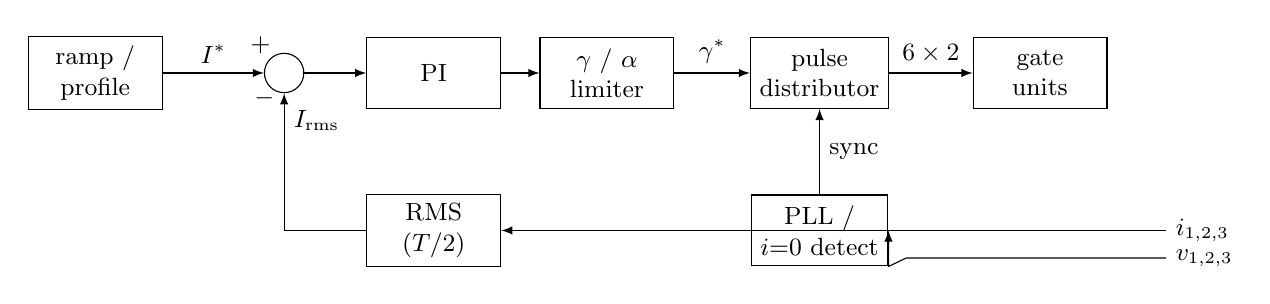
\begin{tikzpicture}[
  blk/.style={draw, minimum height=9mm, minimum width=17mm, align=center,
              font=\small},
  sum/.style={draw, circle, minimum size=5mm, inner sep=0pt, font=\small},
  sig/.style={->, >=latex},
  font=\small]
\node[blk] (ramp) at (0,0) {ramp /\\profile};
\node[sum] (sum) at (2.4,0) {};
\node[blk] (pi) at (4.3,0) {PI};
\node[blk] (lim) at (6.5,0) {$\gamma$ / $\alpha$\\limiter};
\node[blk] (dist) at (9.2,0) {pulse\\distributor};
\node[blk] (gu) at (12.0,0) {gate\\units};
\node[blk] (pll) at (9.2,-2.0) {PLL /\\$i{=}0$ detect};
\node[blk] (rms) at (4.3,-2.0) {RMS\\($T/2$)};
% signals
\draw[sig] (ramp) -- node[above]{$I^\ast$} (sum);
\draw[sig] (sum) -- (pi);
\draw[sig] (pi) -- (lim);
\draw[sig] (lim) -- node[above]{$\gamma^\ast$} (dist);
\draw[sig] (dist) -- node[above]{$6\times2$} (gu);
\draw[sig] (pll) -- node[right]{sync} (dist);
\draw[sig] (rms) -| node[pos=0.9,right]{$I_\mathrm{rms}$} (sum);
\node at (2.15,-0.32) {$-$};
\node at (2.1,0.35) {$+$};
% plant inputs
\draw[sig] (13.6,-2.0) node[right]{$i_{1,2,3}$} -- (rms -| 13.6,0) -- (rms);
\draw[sig] (13.6,-2.35) -- (10.3,-2.35) -- (pll.east |- pll.south east) -- (pll.east);
\node[right] at (13.6,-2.35) {$v_{1,2,3}$};
\end{tikzpicture}
\caption{Control and firing structure of a current-limited soft starter.
The PI regulator commands the hold-off angle $\gamma$; the pulse
distributor generates the six gate signals with double pulsing
(\ang{60}-shifted repeat pulse), synchronized to the line PLL and to the
device current-zero detectors.}
\label{softstart:fig:controlbd}
\end{figure}

Additional logic layers found in industrial products: firing symmetry
supervision (equal positive/negative half-cycle volt-seconds, anti-DC),
kick-start sequencing, transition to full conduction and bypass closure
(the thyristors are kept gated while the bypass closes, so the contactor
never makes the current), and soft-stop ramp-down with the same current
loop. Shorted-thyristor detection is obtained cheaply by monitoring the
voltage across each pair: a device that shows no blocking interval within a
half cycle is declared failed.

%=====================================================================
\section{Power Levels and Device Selection}
%=====================================================================

\subsection{Low-voltage range (\SIrange{200}{690}{\volt})}

LV soft starters are catalogue products from roughly \SI{5}{\kilo\watt} up to
about \SIrange{1}{2}{\mega\watt} (rated currents up to
\SIrange{1600}{2100}{\ampere} at \SI{400}{\volt}--\SI{690}{\volt}). The upper
bound is set by the practicality of LV cabling and switchgear rather than by
the semiconductors. Devices are phase-control thyristors in disc (press-pack)
or module packages with blocking voltages of:
\begin{itemize}
  \item \SIrange{1200}{1600}{\volt} class for \SI{400}{\volt} networks,
  \item \SIrange{1800}{2200}{\volt} class for \SI{690}{\volt} networks,
\end{itemize}
i.e., a repetitive blocking voltage $V_\mathrm{DRM}$ of at least 2--2.5 times
the peak line-to-line voltage, so that normal switching surges are absorbed
without relying on the varistors.

\subsection{Medium-voltage range (\SIrange{2.3}{15}{\kilo\volt})}

MV soft starters cover motors from a few hundred kilowatts to several tens of
megawatts at standard levels of 2.3, 3.3, 4.16, 6.0/6.6, 10/11, and
13.8\,\si{\kilo\volt}. Since single phase-control thyristors are available up
to about \SIrange{6.5}{8.5}{\kilo\volt} blocking, each ``switch'' becomes a
\emph{series string} of $N$ anti-parallel pairs per phase, usually with $N+1$
redundancy so that one shorted device does not force a shutdown. For example,
a \SI{6.6}{\kilo\volt} starter (peak line-to-line \SI{9.3}{\kilo\volt}) built
with \SI{6.5}{\kilo\volt}-class devices and a design utilization of
\SI{2.5}{\kilo\volt} per device uses 4--5 devices per direction per phase.
Series operation is what makes voltage-sharing networks --- and therefore
snubbers --- a first-order design item at MV, as discussed in
Section~\ref{softstart:sec:snubbers}.

Typical MV applications: boiler feed and cooling water pumps, induced/forced
draft fans, refrigeration and gas compressors, SAG/ball mill auxiliaries,
crushers, and large marine or hydro auxiliaries. In many of these, the soft
starter is shared between several motors through a switching scheme (one
starter, $n$ motors), which is economically attractive because the starter
works only a few tens of seconds per start.

\subsection{Thermal duty and utilization categories}

Because the semiconductors work only during the ramp (with bypass), the
rating of a soft starter is inherently a \emph{short-time, repeated-duty}
rating. IEC~60947-4-2, the product standard for AC semiconductor motor
controllers and starters, encodes this in the AC-53 utilization categories;
for example
\begin{center}
AC-53a: 3.5--30 : 50--10
\end{center}
means the starter carries $3.5\,I_e$ for \SI{30}{\second} per start, with
50\,\% on-load duty and 10 starts per hour. The same hardware carries a
higher current rating with a bypass (AC-53b) than without, because the
junction temperature can start each ramp from a lower value. At high power
the practical limit is almost always the number of starts per hour allowed
by the \emph{motor} thermal model, not by the starter.

The relevant device stresses are:
\begin{itemize}
  \item RMS/average current during the ramp (junction temperature excursion,
        checked against the transient thermal impedance $Z_\mathrm{th}(t)$);
  \item surge current $I_\mathrm{TSM}$ and $I^2t$ for coordination with
        fuses or breakers under motor or cable faults;
  \item reapplied $\mathrm{d}v/\mathrm{d}t$ and $\mathrm{d}i/\mathrm{d}t$,
        both mild in line-commutated service but still requiring snubbing,
        as discussed next.
\end{itemize}

%=====================================================================
\section{Interaction with Supply and Motor}
%=====================================================================

During the ramp the phase-controlled currents contain low-order odd
harmonics (5th, 7th, 11th, \dots) and, at large firing angles with
discontinuous conduction, significant higher-order content; the starter also
notches the supply voltage at the commutation instants. Because this lasts
only for the ramp duration (seconds), harmonic standards treat it as a
short-duration emission and it is rarely a compliance problem; it can,
however, disturb sensitive loads on weak feeders, and capacitor banks on the
same bus must not be switched during the ramp (resonance excitation).

On the motor side, reduced-voltage non-sinusoidal supply produces additional
rotor losses and, at large $\alpha$, a torque ripple at $6\times$ line
frequency plus possible subharmonic pulsations under asymmetric firing.
Modern starters symmetrize the firing between the two half-waves precisely
to avoid DC components in the motor current, which would otherwise cause
braking torque and transformer-like saturation effects. Extended operation
at partial voltage (e.g., misused ``energy-saver'' modes) increases motor
heating and is not recommended; the soft starter should be seen strictly as
a starting/stopping device.

%=====================================================================
\section{Snubbers in Soft-Starter Applications}
\label{softstart:sec:snubbers}
%=====================================================================

\subsection{Why snubbers are needed}

Although the soft starter is a line-commutated converter with mild switching
stresses, three mechanisms make snubbers mandatory:

\begin{enumerate}
  \item \textbf{Static and reapplied $\mathrm{d}v/\mathrm{d}t$.} A
        phase-control thyristor can be triggered spuriously by displacement
        current through its center junction capacitance if the anode voltage
        rises too fast. Datasheet critical values are typically
        \SIrange{500}{1000}{\volt\per\micro\second} for a blocking device
        and much lower during the turn-off interval $t_q$, when reapplied
        $\mathrm{d}v/\mathrm{d}t$ can re-fire a device that has just
        commutated. In the soft starter, every current zero of an outgoing
        thyristor is followed by a step of instantaneous line voltage across
        the pair; through the supply stray inductance this step arrives as a
        fast, ringing edge unless it is snubbed. A spurious turn-on in an
        anti-parallel pair short-circuits nothing by itself, but it destroys
        the voltage control, can create DC components in the motor current,
        and in a series string it overvoltages the remaining devices.
  \item \textbf{Reverse-recovery (commutation) overvoltage.} At each current
        zero the outgoing thyristor sweeps out its recovered charge; the
        recovery current snapping off in the loop inductance produces a
        voltage overshoot across the device. In line-commutated service the
        $\mathrm{d}i/\mathrm{d}t$ at the current zero is low
        ($\omega \hat{I}$, a few \si{\ampere\per\micro\second}), so
        $I_\mathrm{RM}$ is modest, but with the large disc devices used at
        high power the recovered charge is still tens of millicoulombs and
        the overshoot must be damped.
  \item \textbf{Line-borne transients and voltage sharing.} The starter
        hangs directly on the distribution bus and sees contactor switching
        surges, capacitor-bank energization transients, and lightning-borne
        surges. In MV series strings, the snubber additionally performs
        \emph{dynamic voltage grading}: it equalizes the voltage across
        devices that turn off with slightly different recovered charges or
        turn on with different delay times.
\end{enumerate}

\subsection{RC snubber across the pair}

Since at any instant at most one device of an anti-parallel pair is
blocking, a single RC snubber connected across the pair protects both
directions (Fig.~\ref{softstart:fig:snubber}). A metal-oxide varistor (MOV) in
parallel clamps energy-rich surges that the RC cannot absorb.

\begin{figure}[htb]
\centering
\begin{circuitikz}[scale=1.0, transform shape]
\draw (0,2) node[left]{line} to[short] (1,2);
% pair
\draw (1,2) -- (1,3) to[Ty] (4,3) -- (4,2);
\draw (1,2) -- (1,1);
\draw (4,1) to[Ty] (1,1);
\draw (4,1) -- (4,2);
\draw (4,2) to[short] (6.5,2) node[right]{motor};
% RC snubber
\draw (1,2) -- (1,-0.4) to[R, l_=$R_\mathrm{s}$] (2.9,-0.4)
      to[C, l_=$C_\mathrm{s}$] (4,-0.4) -- (4,2);
% MOV
\draw (1,-0.4) -- (1,-1.8) to[varistor, l_=MOV] (4,-1.8) -- (4,-0.4);
\end{circuitikz}
\caption{Anti-parallel thyristor pair with RC snubber and metal-oxide
varistor. One RC network per pair suffices, since only one device blocks at
a time.}
\label{softstart:fig:snubber}
\end{figure}

\paragraph{Sizing model.} The design case is a voltage step $V_0$ (worst
case: the instantaneous line-to-line voltage at a current zero, up to
$\hat{V}_\mathrm{LL} = \sqrt{2}\,V_\mathrm{LL}$) applied through the supply
inductance per phase $L_\sigma$ to the $R_\mathrm{s}$--$C_\mathrm{s}$
branch. With the device blocking, the series $L_\sigma R_\mathrm{s}
C_\mathrm{s}$ circuit gives:
\begin{align}
  \omega_0 &= \frac{1}{\sqrt{L_\sigma C_\mathrm{s}}}, &
  Z_0 &= \sqrt{\frac{L_\sigma}{C_\mathrm{s}}}, &
  \zeta &= \frac{R_\mathrm{s}}{2 Z_0},
\end{align}
\begin{equation}
  \left.\frac{\mathrm{d}v_\mathrm{T}}{\mathrm{d}t}\right|_{t=0}
  = \frac{R_\mathrm{s} V_0}{L_\sigma},
  \qquad
  \left.\frac{\mathrm{d}v_\mathrm{T}}{\mathrm{d}t}\right|_\mathrm{peak}
  \approx k(\zeta)\, \omega_0 V_0 ,
  \label{softstart:eq:dvdt}
\end{equation}
where $k(\zeta) \approx 1$ for $\zeta \approx 0.5\ldots0.7$. The classical
optimization (McMurray \cite{mcmurray1972}) trades peak voltage against peak
$\mathrm{d}v/\mathrm{d}t$; for soft starters, where the switching frequency
is the line frequency and snubber loss is a secondary concern, a simple and
robust recipe is:

\begin{enumerate}
  \item Choose $C_\mathrm{s}$ so that
        $\omega_0 V_0 \le (0.2\ldots0.3)\times
        (\mathrm{d}v/\mathrm{d}t)_\mathrm{crit}$,
        keeping a large margin because the reapplied-$\mathrm{d}v/\mathrm{d}t$
        capability right after commutation is far below the static datasheet
        value.
  \item Choose $R_\mathrm{s} = 2\zeta Z_0$ with $\zeta \approx 0.5\ldots0.7$
        for near-critical damping of the ring.
  \item Check the additional overshoot due to recovery:
        $\Delta V \approx I_\mathrm{RM} Z_0$, and verify
        $V_\mathrm{peak} \le V_\mathrm{DRM}$ with margin.
  \item Check the snubber discharge current at thyristor turn-on,
        $\hat{I}_\mathrm{dis} \approx V_0 / R_\mathrm{s}$, against the gate
        area's $\mathrm{d}i/\mathrm{d}t$ capability (this sets a lower bound
        on $R_\mathrm{s}$).
  \item Rate the resistor for the cyclic energy
        $P_{R} \approx f_\mathrm{line}\, C_\mathrm{s} V_0^2$
        (charge and discharge once per half cycle per polarity) with a
        pulse-rated (wirewound or thick-film) part.
\end{enumerate}

\subsection{Worked example: \SI{690}{\volt}, \SI{1}{\mega\watt} starter}

Motor: \SI{1}{\mega\watt}, \SI{690}{\volt}, $\eta = 0.96$,
$\cos\varphi = 0.85$, hence $I_N \approx \SI{1025}{\ampere}$; current-limit
start at $3.5\,I_N \approx \SI{3.6}{\kilo\ampere}$ RMS for
\SI{30}{\second}. Supply: \SI{2}{\mega\voltampere} transformer,
$u_k = 6\,\%$:
\begin{equation}
  L_\sigma = \frac{u_k V_\mathrm{LL}^2}{\omega S}
  = \frac{0.06 \times 690^2}{314 \times 2\times10^6}
  \approx \SI{45}{\micro\henry}\ \text{per phase}.
\end{equation}
Worst-case step: $V_0 = \sqrt{2}\times 690 \approx \SI{976}{\volt}$.
Device: \SI{2200}{\volt}-class phase-control disc thyristor,
$(\mathrm{d}v/\mathrm{d}t)_\mathrm{crit} = \SI{1000}{\volt\per\micro\second}$.

Choosing $C_\mathrm{s} = \SI{0.5}{\micro\farad}$:
\begin{equation}
  \omega_0 = \frac{1}{\sqrt{45\,\mu \times 0.5\,\mu}}
  \approx \SI{211}{\kilo\radian\per\second}, \qquad
  Z_0 = \sqrt{\frac{45\,\mu}{0.5\,\mu}} \approx \SI{9.5}{\ohm},
\end{equation}
\begin{equation}
  \left(\frac{\mathrm{d}v}{\mathrm{d}t}\right)_\mathrm{peak}
  \approx \omega_0 V_0 \approx \SI{206}{\volt\per\micro\second}
  \quad (\approx 20\,\% \text{ of the static limit; ample margin for } t_q).
\end{equation}
Damping: $R_\mathrm{s} = 2 \times 0.5 \times 9.5 \approx \SI{10}{\ohm}$
($\zeta = 0.5$); initial slope $R_\mathrm{s}V_0/L_\sigma =
\SI{217}{\volt\per\micro\second}$, consistent. Recovery overshoot with
$I_\mathrm{RM} \approx \SI{60}{\ampere}$ (low
$\mathrm{d}i/\mathrm{d}t$, large device):
$\Delta V \approx 60 \times 9.5 \approx \SI{570}{\volt}$, so
$V_\mathrm{peak} \lesssim 1.2\,V_0 + \Delta V \approx \SI{1.75}{\kilo\volt}
< \SI{2.2}{\kilo\volt}$. Snubber discharge at turn-on:
$976/10 \approx \SI{98}{\ampere}$ superimposed on the load
$\mathrm{d}i/\mathrm{d}t$ --- negligible for a disc device. Resistor power:
\begin{equation}
  P_R \approx f C_\mathrm{s} V_0^2
  = 50 \times 0.5\times10^{-6} \times 976^2 \approx \SI{24}{\watt}
\end{equation}
per pair; a \SI{50}{\watt} pulse-rated wirewound resistor is adequate. Note
that after bypass the snubber still sits across the (open) pair in parallel
with the closed contactor, so it is unstressed in run; without bypass it
dissipates $P_R$ continuously.

\subsection{Series strings in MV starters: grading networks}

In an MV starter each phase switch is a string of $N$ pairs, and the total
blocking voltage must divide acceptably among devices that are not
identical. Two networks are used per device (or per pair):

\begin{itemize}
  \item \textbf{Static grading resistor} $R_\mathrm{p}$ (tens to hundreds of
        \si{\kilo\ohm}) in parallel with each device, sized so that its
        current is 3--10 times the maximum spread of device leakage
        currents. It fixes the off-state (DC and \SI{50}{\hertz}) sharing.
  \item \textbf{Dynamic grading = RC snubber} across each device. During
        commutation, devices recover with different charges; the device that
        recovers first must absorb the voltage until the others follow. The
        sharing error is
        \begin{equation}
          \Delta V \approx \frac{\Delta Q_\mathrm{rr}}{C_\mathrm{s}},
          \label{softstart:eq:grading}
        \end{equation}
        where $\Delta Q_\mathrm{rr}$ is the maximum recovered-charge
        mismatch within the string (from datasheet spread or from lot
        selection). Equation~\eqref{softstart:eq:grading} typically dominates the
        choice of $C_\mathrm{s}$ at MV: with
        $\Delta Q_\mathrm{rr} = \SI{2}{\milli\coulomb}$ and an allowed
        imbalance of \SI{500}{\volt}, $C_\mathrm{s} \geq
        \SI{4}{\micro\farad}$ would be needed --- which is why MV designs
        select/match devices for recovered charge, accept larger per-device
        margins, or use larger snubbers than the $\mathrm{d}v/\mathrm{d}t$
        criterion alone would suggest.
\end{itemize}

The same string design rules as in HVDC valves apply in miniature: firing
delay spread converts directly into transient overvoltage on the last
device to fire, which the snubber must buffer; hence the preference for
fiber-optic gating with tightly controlled delays at MV.

\subsection{Varistors and protection coordination}

MOVs across each pair (LV) or each device/string section (MV) clamp
line-borne surges. Coordination is straightforward:
\begin{equation}
  V_\mathrm{clamp,max} < V_\mathrm{DRM}
  \quad\text{and}\quad
  V_\mathrm{MOV,cont} > \hat{V}_\mathrm{LL}\times\text{margin},
\end{equation}
with the RC snubber handling the fast front (limiting
$\mathrm{d}v/\mathrm{d}t$) and the MOV the energy. In addition,
overvoltage-triggered firing (break-over diode or active crowbar gating) is
often implemented at MV: if the string voltage approaches the design limit,
the thyristors are deliberately fired into conduction, which is a safe state
for a device feeding a motor.

\subsection{Practical remarks}

\begin{itemize}
  \item \textbf{Leakage path.} The RC network conducts at line frequency even
        with gating inhibited: the motor terminals are never galvanically
        dead through a soft starter. An isolating contactor or disconnector
        upstream is mandatory for safe maintenance, and this is reflected in
        the product standards.
  \item \textbf{Capacitor technology.} Film capacitors (dry, self-healing,
        AC-rated) with low ESL; the loop starter--snubber must be short
        because stray inductance inside the snubber loop defeats its
        purpose.
  \item \textbf{Resistors.} Pulse-withstanding types; the peak pulse power
        $V_0^2/R_\mathrm{s}$ (tens of kilowatts for microseconds) is the
        sizing quantity together with the average $P_R$.
  \item \textbf{No snubber is not an option.} Unlike IGBT converters, where
        snubberless designs are common, phase-control thyristors in direct
        line service without RC networks will sooner or later fire on a
        network transient. The snubber here is a protection element, not an
        efficiency optimization.
\end{itemize}

%=====================================================================
\section{Soft Starter versus VFD}
%=====================================================================

The choice at high power is usually between a soft starter and a
medium-voltage VFD:

\begin{itemize}
  \item If the process is genuinely fixed-speed, the soft starter wins on
        cost (roughly 3--10 times cheaper), footprint, efficiency (after
        bypass the path is metallic), reliability, and harmonic behavior
        (transient emission only).
  \item If the load can exploit variable speed (throttled pumps and fans),
        the VFD's energy savings normally dominate the economics despite the
        higher cost.
  \item The VFD starts the motor at rated flux with up to rated torque at
        $\leq I_N$ line current; the soft starter fundamentally cannot
        provide high torque at low current
        (Eq.~\eqref{softstart:eq:v2}). For high-inertia or high-breakaway loads at MV,
        this is often the deciding technical argument.
\end{itemize}

A hybrid practice at MV is one VFD used as a \emph{starting drive} for
several motors, synchronizing each motor to the line and transferring it;
the soft starter is the simpler and far more common realization of the same
``start-then-bypass'' idea.

%=====================================================================
\section{Conclusion}
%=====================================================================

The thyristor soft starter is a minimal, robust, line-commutated AC voltage
controller that solves the starting-transient problem of fixed-speed
induction motors from tens of kilowatts (LV catalogue products up to about
\SIrange{1}{2}{\mega\watt}) to tens of megawatts (MV designs with
series-connected thyristor strings). Its power semiconductors operate in a
short-time, repeated duty defined by IEC~60947-4-2 utilization categories,
and are almost always bypassed in run. Snubbers are an integral protection
element in these applications: RC networks across each anti-parallel pair
limit the reapplied $\mathrm{d}v/\mathrm{d}t$ at every line commutation,
damp recovery-driven ringing against the supply inductance, and --- in MV
series strings --- provide the dynamic voltage grading without which series
operation is not feasible. Their sizing is undemanding at LV (fractions of a
microfarad, tens of ohms, tens of watts) but becomes a first-order design
constraint at MV, where recovered-charge mismatch sets the capacitance and
device matching becomes part of the snubber design.

%=====================================================================

